\documentclass{article}

\usepackage{booktabs}
\usepackage{tabularx}
\usepackage{hyperref}
\usepackage{graphicx}
\usepackage[a4paper, margin=0.75in]{geometry}
\usepackage{subcaption}
\usepackage{float}


\hypersetup{
    colorlinks=true,       % false: boxed links; true: colored links
    linkcolor=red,          % color of internal links (change box color with linkbordercolor)
    citecolor=green,        % color of links to bibliography
    filecolor=magenta,      % color of file links
    urlcolor=cyan           % color of external links
}

\title{Hazard Analysis\\\progname}

\author{\authname}

\date{}

%% Comments

\usepackage{color}

\newif\ifcomments\commentstrue %displays comments
%\newif\ifcomments\commentsfalse %so that comments do not display

\ifcomments
\newcommand{\authornote}[3]{\textcolor{#1}{[#3 ---#2]}}
\newcommand{\todo}[1]{\textcolor{red}{[TODO: #1]}}
\else
\newcommand{\authornote}[3]{}
\newcommand{\todo}[1]{}
\fi

\newcommand{\wss}[1]{\authornote{magenta}{SS}{#1}} 
\newcommand{\plt}[1]{\authornote{cyan}{TPLT}{#1}} %For explanation of the template
\newcommand{\an}[1]{\authornote{cyan}{Author}{#1}}

%% Common Parts

\newcommand{\progname}{Software Engineering} % PUT YOUR PROGRAM NAME HERE
\newcommand{\teamname}{EvENGage}
\newcommand{\authname}{Team 4, \teamname
\\ Virochaan Ravichandran Gowri
\\ Omar Al-Asfar
\\ Rayyan Suhail
\\ Ibrahim Quraishi
\\ Mohammad Mahdi Mahboob} % AUTHOR NAMES

\newcommand{\prjdesc}{MES Event Management Registration, Administration, and Survey Analytics}

\usepackage{hyperref}
    \hypersetup{colorlinks=true, linkcolor=blue, citecolor=blue, filecolor=blue,
                urlcolor=blue, unicode=false}
    \urlstyle{same}



\begin{document}

\maketitle
\thispagestyle{empty}

~\newpage

\pagenumbering{roman}

\begin{table}[hp]
\caption{Revision History} \label{TblRevisionHistory}
\begin{tabularx}{\textwidth}{llX}
\toprule
\textbf{Date} & \textbf{Developer(s)} & \textbf{Change}\\
\midrule
09-25-2025 & Rayyan Suhail & Added Component Overview and Boundaries\\
09-29-2025 & Rayyan Suhail & FMEA Added\\
... & ... & ...\\
\bottomrule
\end{tabularx}
\end{table}

~\newpage

\tableofcontents

~\newpage

\pagenumbering{arabic}

\wss{You are free to modify this template.}

\section{Introduction}

\wss{You can include your definition of what a hazard is here.}

\section{Scope and Purpose of Hazard Analysis}

\wss{You should say what \textbf{loss} could be incurred because of the
hazards.}

\section{System Boundaries and Components}

The proposed platform will be utilized by the McMaster Engineering Society (MES)
as a centralized event management system and survey feedback collection system.
The system boundary includes all the functionality required to build and render
custom forms, manage event registrations and waivers, check-ins, deliver
notifications, and build analytics dashboards.

\subsection{System Boundaries}

\begin{itemize}
    \item \textbf{In Scope}: Administrator and student web and mobile interfaces, 
    form builder and renderer, registration and waiver processing, check-in and QR verification, 
    attendee overview dashboard, analytics and reporting, notifications, authentication and authorization, 
    and internal data storage.
    
    \item \textbf{Not Covered}: Third-party services like university single sign-on (SSO), 
    third-party email/SMS portals, and payment sites. These are treated as outside dependencies, 
    with interactions regulated through integration adapters.
    
    \item \textbf{Environment}: The system is web-based, compatible with major browsers, 
    and supports portable devices (iOS and Android). Its operation requires steady internet connectivity, 
    although it offers minimal offline capability for the check-in process.
\end{itemize}

\subsection{Component Overview}

The system can be divided into the following major components for hazard analysis:

\subsubsection{Admin Web Application}
Provides administrators with tools to build forms, configure events, manage attendees, and view analytics.

\subsubsection{End-User Application (Web/Mobile)}
Interface for students to register for events and submit feedback surveys.

\subsubsection{Custom Form Builder and Renderer}
Schema-based system to define and display registration and feedback forms, including branching and conditional logic.

\subsubsection{Registration Form Manager}
Handles the creation and processing of registration forms, ensuring that event-specific data is collected accurately.

\subsubsection{Attendee Overview Dashboard}
Provides administrators with a consolidated view of registrations and attendee details for an event.

\subsubsection{Analytics and Reporting}
Generates data visualizations and exportable reports based on registration and survey responses, enabling event planning and improvement.

\subsubsection{Data Storage Layer}
Stores form schemas, form responses, and attendee information using structured databases and JSON-based storage.

\subsubsection{External Integration Adapters}
Interfaces with required external systems such as university single sign-on (SSO) and email services to support core functionality.




\section{Critical Assumptions}

\wss{These assumptions that are made about the software or system.  You should
minimize the number of assumptions that remove potential hazards.  For instance,
you could assume a part will never fail, but it is generally better to include
this potential failure mode.}

\section{Failure Mode and Effects Analysis (FMEA)}

The following section provides a breakdown of the Failure Modes and Effects Analysis (FMEA) for the system. Each component is evaluated for potential failures, their impact on system operation, possible causes, methods of detection, and recommended actions. This analysis ensures that hazards affecting event registration, form processing, check-ins, and analytics are identified early and mitigated through targeted safety and reliability requirements.
\begin{figure}[H]
\begin{subfigure}{\textwidth}
    \centering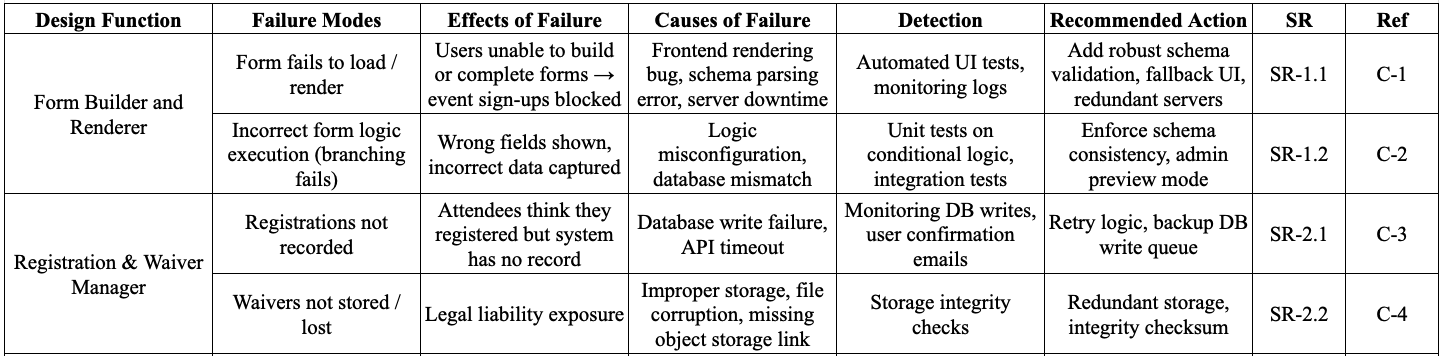
\includegraphics[width=\textwidth]{FMEA_images/FMEA_1.png} 
    \caption{Fig. 1: FMEA Table Part 1}
\end{subfigure}

\begin{subfigure}{\textwidth}
    \centering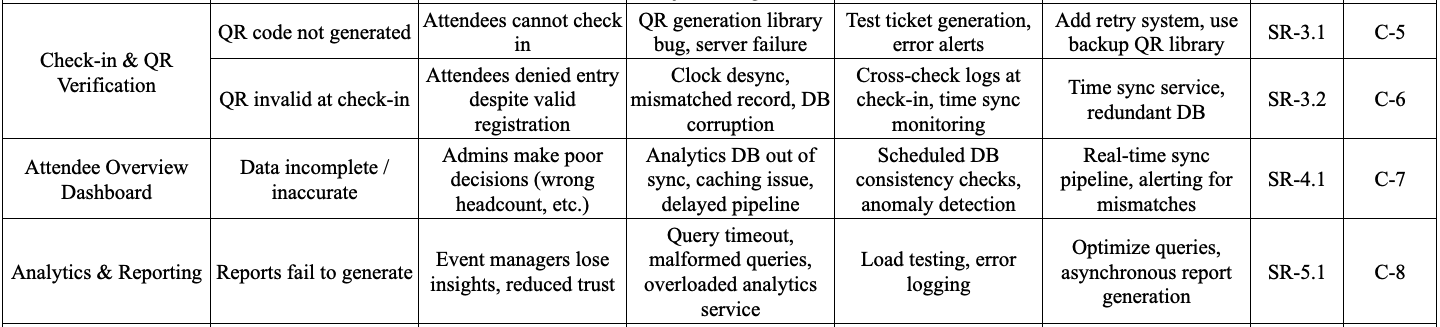
\includegraphics[width=\textwidth]{FMEA_images/FMEA_2.png}
    \caption{Fig. 2: FMEA Table Part 2}
\end{subfigure}

\begin{subfigure}{\textwidth}
    \centering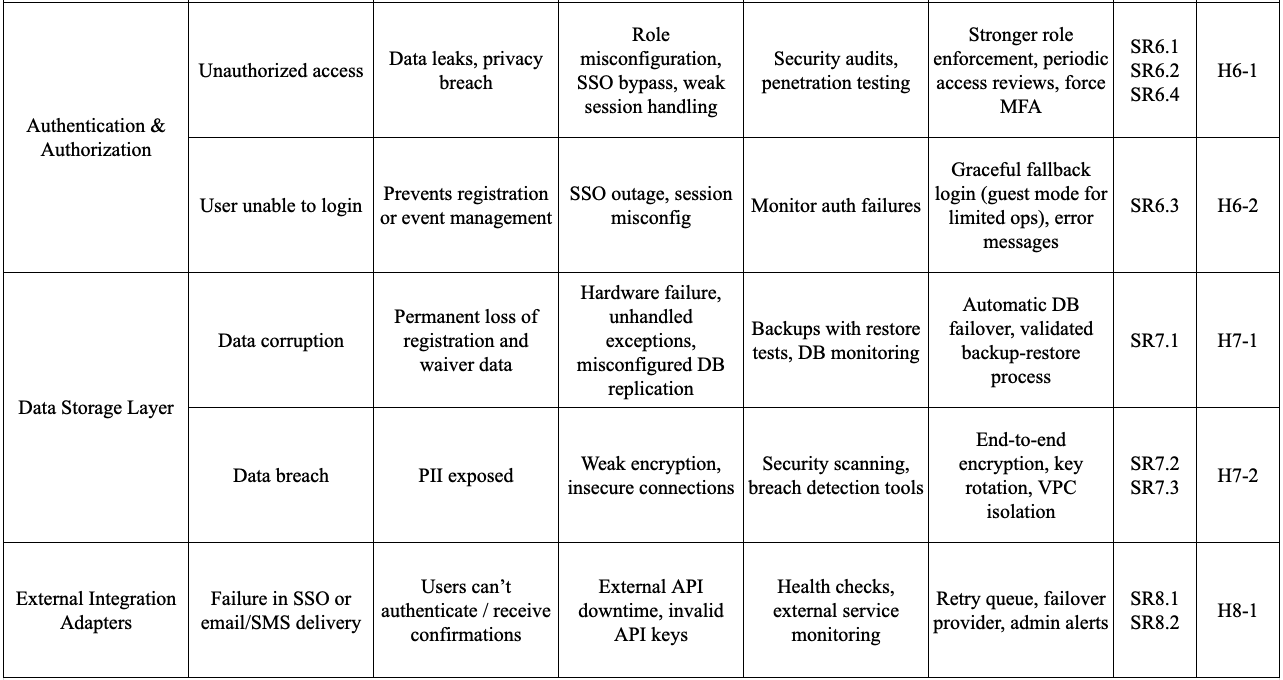
\includegraphics[width=\textwidth]{FMEA_images/FMEA_3.png}
    \caption{Fig. 3: FMEA Table Part 3}
\end{subfigure}
\end{figure}



\section{Safety and Security Requirements}

The following safety and security requirements were derived from the Failure Mode and Effects Analysis (FMEA). 
They represent newly discovered requirements that should also be included in the Software Requirements Specification (SRS).

\subsection{Form Builder \& Renderer}
\begin{itemize}
    \item \textbf{SR1.1}: The system shall validate all form schemas before rendering to prevent failures.
    \item \textbf{SR1.2}: The system shall enforce schema consistency across frontend and database logic.
    \item \textbf{SR1.3}: The system shall provide redundant servers or fallback UI during outages.
\end{itemize}

\subsection{Registration \& Waiver Manager}
\begin{itemize}
    \item \textbf{SR2.1}: The system shall implement retry logic and backup queues for database writes.
    \item \textbf{SR2.2}: The system shall send confirmation receipts after successful registration.
    \item \textbf{SR2.3}: The system shall store waiver data redundantly with integrity checks.
\end{itemize}

\subsection{Check-In \& QR Verification}
\begin{itemize}
    \item \textbf{SR3.1}: The system shall provide retry and backup QR code generation.
    \item \textbf{SR3.2}: The system shall enforce synchronized clocks across all check-in endpoints.
\end{itemize}

\subsection{Attendee Overview Dashboard}
\begin{itemize}
    \item \textbf{SR4.1}: The system shall continuously sync databases to prevent inconsistencies.
    \item \textbf{SR4.2}: The system shall implement anomaly detection to detect corrupted or missing data.
\end{itemize}

\subsection{Analytics \& Reporting}
\begin{itemize}
    \item \textbf{SR5.1}: The system shall support asynchronous report generation to handle load.
\end{itemize}

\subsection{Authentication \& Authorization}
\begin{itemize}
    \item \textbf{SR6.1}: The system shall enforce role-based permissions and periodic access reviews.
    \item \textbf{SR6.2}: The system shall support multi-factor authentication for administrators.
    \item \textbf{SR6.3}: The system shall provide a fallback login during SSO outages.
    \item \textbf{SR6.4}: The system shall monitor and log failed login attempts and alert admins.
\end{itemize}

\subsection{Data Storage Layer}
\begin{itemize}
    \item \textbf{SR7.1}: The system shall back up databases automatically and validate restore processes.
    \item \textbf{SR7.2}: The system shall encrypt data at rest and rotate encryption keys regularly.
    \item \textbf{SR7.3}: The system shall store sensitive data in a secure isolated environment (VPC).
\end{itemize}

\subsection{External Integration Adapters}
\begin{itemize}
    \item \textbf{SR8.1}: The system shall implement retry queues and failover providers for external APIs.
    \item \textbf{SR8.2}: The system shall continuously monitor third-party service health and alert admins.
\end{itemize}


\section{Roadmap}

The hazard analysis identified several safety and security requirements. Within the capstone timeline, the focus will be on core reliability and usability features, including schema validation and fallback UI (SR1.1), reliable registration storage (SR2.1), QR code generation fallback (SR3.1), dashboard synchronization (SR4.1), and authentication fallback handling (SR6.2). More advanced requirements such as multi-factor authentication (SR6.1), scalable analytics (SR5.1), stronger data protection mechanisms (SR7.1, SR7.2), and redundant integration failover (SR8.1) are deferred to future development beyond the capstone scope. At project completion, the hazard analysis will be revisited to assess which risks have been mitigated and which requirements should be prioritized for follow-up work.


\newpage{}

\section*{Appendix --- Reflection}

\wss{Not required for CAS 741}

The purpose of reflection questions is to give you a chance to assess your own
learning and that of your group as a whole, and to find ways to improve in the
future. Reflection is an important part of the learning process.  Reflection is
also an essential component of a successful software development process.  

Reflections are most interesting and useful when they're honest, even if the
stories they tell are imperfect. You will be marked based on your depth of
thought and analysis, and not based on the content of the reflections
themselves. Thus, for full marks we encourage you to answer openly and honestly
and to avoid simply writing ``what you think the evaluator wants to hear.''

Please answer the following questions.  Some questions can be answered on the
team level, but where appropriate, each team member should write their own
response:


\begin{enumerate}
    \item What went well while writing this deliverable? 
    \item What pain points did you experience during this deliverable, and how
    did you resolve them?
    \item Which of your listed risks had your team thought of before this
    deliverable, and which did you think of while doing this deliverable? For
    the latter ones (ones you thought of while doing the Hazard Analysis), how
    did they come about?
    \item Other than the risk of physical harm (some projects may not have any
    appreciable risks of this form), list at least 2 other types of risk in
    software products. Why are they important to consider?
\end{enumerate}

\end{document}